\textbf{Solución 1:}
    El sistema se alimentará de $220\text{VAC }60\text{Hz}$, la cual será suministrada directamente de un tomacorriente estándar en Perú. Desde el chasis del dispositivo, el usuario podrá energizar o desactivar todos los módulos mediante un botón de encendido y apagado. En cuanto a la seguridad, se ha integrado un botón de parada de emergencia en el mismo chasis para desactivar rápidamente todos los módulos en caso se de la necesidad, ya que cómo se mostró en la sección \ref{sec:CH03_FUNCIONES} , el sistema deberá ser capaz de desenergizarse para evitar dañar al usuario que esté en contacto con el \ac{HW} del sistema. 
    	
    El estado de funcionamiento de los módulos será visible para el usuario mediante un sistema de indicadores LED. Estos LEDs, de colores diferenciados, indicarán si cada uno de los tres dominios principales (Control, Sensores y Actuadores) está energizado y funcionando correctamente. De esta manera, el usuario podrá observar de forma rápida y clara el estado de cada subsistema del dispositivo.
    	
    Para asegurar la correcta disipación del calor generado por los circuitos energizados, el chasis cuenta con un pequeño ventilador y ranuras, que favorezcan la circulación de aire para mantener la temperatura de los componentes dentro de un rango seguro durante su operación. Las perforaciones del chasis son válidas, al estar utilizando una estructura principalmente de chapa. El chasis también dispone de puertos USBs que permiten la conexión directa entre el \ac{HW} y el \ac{SW}, permitiendo la transferencia de datos desde ambos dominios.
        
    En la Figura \ref{fig:sol1_fuera}  se muestra un bosquejo de la vista exterior del concepto propuesto.
    \begin{figure}[H]
        \centering
        \begin{tabularx}{\linewidth}{>{\centering\arraybackslash}X}
            % Fila 1: imagen
            \begin{subfigure}[t]{1\linewidth}
                \centering
                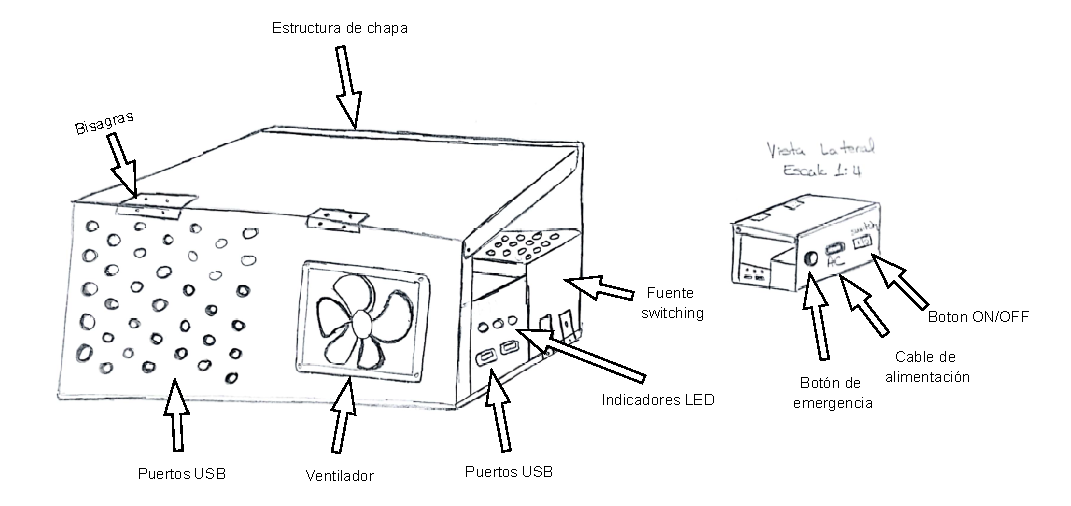
\includegraphics[width=\linewidth]{CHPTRS/CH03_DICON/Fig/CH03_FIG02_CoS/01_CoS_Solucion1porFuera.pdf}
            \end{subfigure}
        \end{tabularx}
        \caption{Concepto 1 - Vista desde afuera del \ac{HW} del sistema}
        \label{fig:sol1_fuera}
    \end{figure}
    
    En el diseño interno del \ac{HW} se ha considerado un sistema de protección mediante fusibles colocados en la sección de entrada de potencia, donde se conecta la alimentación desde el tomacorriente. Estos fusibles protegerán los componentes ante posibles sobrecargas y garantizarán la seguridad del sistema. Además, para optimizar el espacio dentro del chasis, se implementarán conectores o pistas de \ac{PCB}  para distribuir la alimentación a todos los módulos, con la finalidad de no ocupar demasiada área.
    El sistema incluirá circuitos de potencia o \textit{drivers} para alimentar dos motores: uno será el objeto de análisis, mientras que el otro accionará un mecanismo de fijación diseñado para sujetar al motor que se va a caracterizar. Esto requiere como mínimo la incorporación de dos \textit{drivers}, cada uno conectado a los motores \ac{DC}, sólo que uno será controlado mediante accionamientos del usuario, mientras que el otro, que servirá para la estimación, será automatizado con la información que se ingrese en la interfaz al inicio de la estimación. Como se mencionó, el ajuste del motor a la estructura de prueba será manual, y el usuario deberá operar algunos botones para fijar el motor en su lugar mediante un sistema de sujeción similar a un tornillo de banco. Adicionalmente, se integrará un sensor de presencia que verificará que el motor esté correctamente posicionado antes de iniciar el proceso de estimación. Es importante destacar que para la salida del \textit{driver} conectado al motor por analizar, se deberá acoplar unos cables que puedan ser extendibles y que se fijen a las escobillas o cables de alimentación del motor.
    
    Todos los sensores, estos estarán ensamblados por cable a una \ac{PCB} y conectados a la unidad de control, que en este caso a una \ac{SBC}. Cabe señalar que, de todos los sensores, el de velocidad puede no estar en una posición fija, ya que deberá ajustarse en función del tamaño del motor a evaluar. Anteriormente, se presentaron dos tipos de sensores de velocidad, y para esta solución se ha optado por un \textit{encoder} óptico. Este \textit{encoder} estará montado en una estructura ajustable y desplazable que permita fijarlo de manera precisa sobre el eje del motor para asegurar una medición exacta de la velocidad.
    
    Como se trata de una \ac{SBC}, se han tomado en cuenta consideraciones de acondicionamiento para capturar los datos de manera precisa, así como para realizar un preprocesamiento inicial de los datos antes de enviarlos al \ac{SW} del sistema. En cuanto a las comunicaciones con la \ac{SBC}, se utilizará el puerto de comunicación incorporado; no obstante, existe la opción de acondicionar los puertos USBs en caso de que sea necesario.
    
    Para simplificar el boceto de la solución, se ha dividido el área de la \ac{PCB} en grandes rectángulos, que representan cada una de las zonas funcionales del sistema, debido a que no se busca saturar el dibujo con geometrías complejas de componentes electrónicos. A continuación, en la Figura \ref{fig:sol1_dentro} se muestra el bosquejo de vista interior.
    \begin{figure}[H]
        \centering
        \begin{tabularx}{\linewidth}{>{\centering\arraybackslash}X}
            % Fila 1: imagen
            \begin{subfigure}[t]{0.8\linewidth}
                \centering
                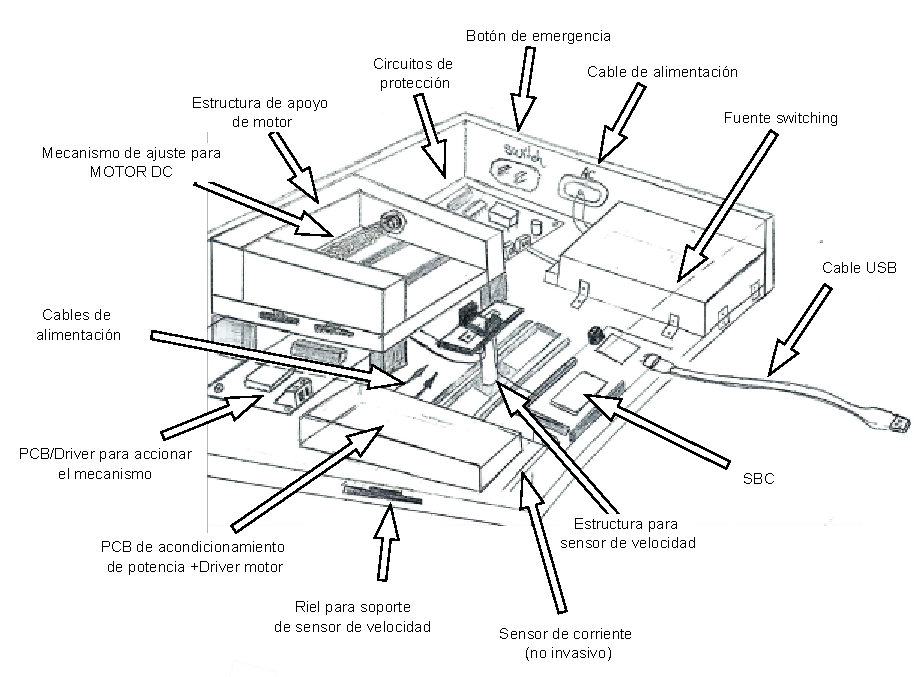
\includegraphics[width=\linewidth]{CHPTRS/CH03_DICON/Fig/CH03_FIG02_CoS/02_CoS_Solucion1porDentro.pdf}
            \end{subfigure}
        \end{tabularx}
        \caption{Concepto 1 - Vista desde adentro del \ac{HW} del sistema}
        \label{fig:sol1_dentro}
    \end{figure}
       
    Para el acople de \textit{encoder} se pretende diseñar un disco ranurado dado que el sensor utilizado es de infrarrojos. Cada que el disco deje pasar la luz infrarroja se registrará una cuenta, en la unidad de control. Esta data se recopilará y se filtrará digitalmente para eliminar el ruido y falsas mediciones  debido al error presente al detectar los flancos con este tipo de sensor.
    A continuación se presenta la posición del soporte del sensor de velocidad en la Figura \ref{fig:acople_op}
    \begin{figure}[H]
        \centering
        \begin{tabularx}{\linewidth}{>{\centering\arraybackslash}X}
            % Fila 1: imagen
            \begin{subfigure}[t]{0.8\linewidth}
                \centering
                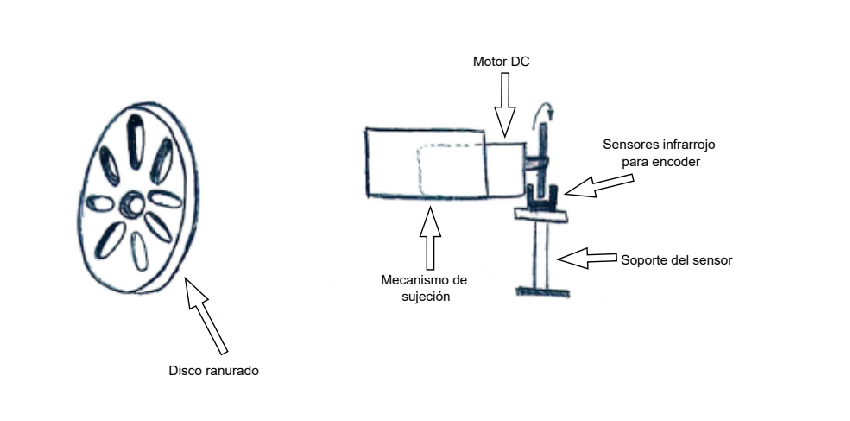
\includegraphics[width=\linewidth]{CHPTRS/CH03_DICON/Fig/CH03_FIG02_CoS/03_CoSAcopleOptico1.pdf}
            \end{subfigure}
        \end{tabularx}
        \caption{Acople de \textit{encoder} óptico}
        \label{fig:acople_op}
    \end{figure}
    
    El mecanismo de ajuste utilizará un tornillo sin fin en combinación con una tuerca fija en uno de sus extremos, de modo que, al girar, este sistema genere la presión necesaria para asegurar el motor \ac{DC}. Este giro será efectuado por un motor \ac{DC} acoplado al eje del tornillo sin fin. Aunque la mayor parte de la estructura se diseñará en chapa metálica, se considera la fabricación de algunos elementos y sus sujeciones mediante impresión 3D. Además, se emplearán elementos mecánicos, como tornillos, para las demás sujeciones de estos componentes. Adicionalmente, para el apoyo del motor se deberá diseñar unas ranuras por donde se desplazará la pared móvil que apretará al motor. En la  Figura \ref{fig:detalle1} se muestra las uniones del soporte donde se apoyará el motor a analizar.
    \begin{figure}[!ht]
        \begin{tabularx}{\linewidth}{*{2}{>{\centering\arraybackslash}X}}
            % FILA-1 (imágenes superiores)
            \begin{subfigure}[t]{0.45\textwidth}
                \centering
                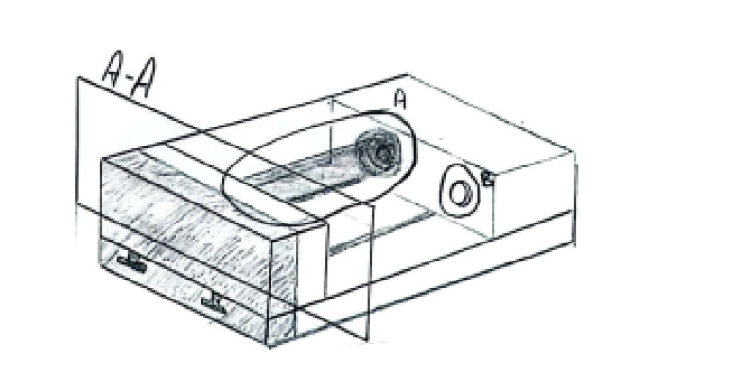
\includegraphics[width=.9\linewidth]{CHPTRS/CH03_DICON/Fig/CH03_FIG02_CoS/04a_CoSDibujoDeMecanismo.pdf}
            \end{subfigure}
            &
            \begin{subfigure}[t]{0.45\textwidth}
                \centering
                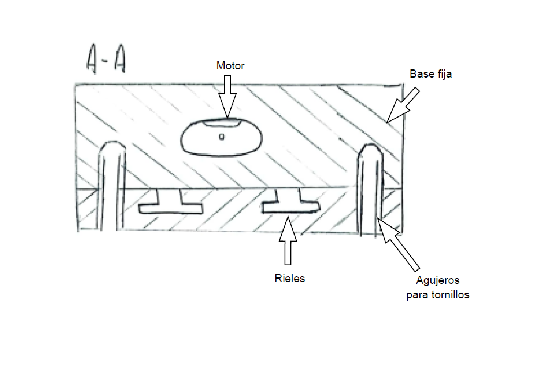
\includegraphics[width=.9\linewidth]{CHPTRS/CH03_DICON/Fig/CH03_FIG02_CoS/04b_CoSDibujoDeSeccion.pdf}
            \end{subfigure}
            \\
            % FILA-2 (imágenes inferiores)
            \begin{subfigure}[t]{0.45\textwidth}
                \centering
                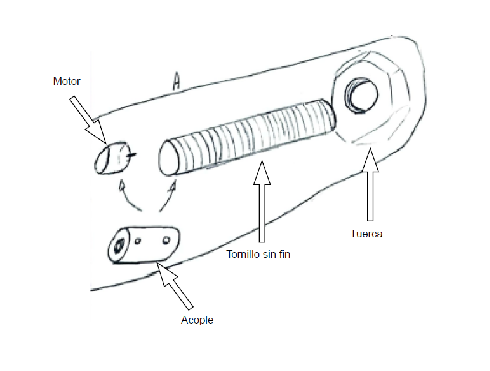
\includegraphics[width=.9\linewidth]{CHPTRS/CH03_DICON/Fig/CH03_FIG02_CoS/04c_CoSDibujosDeSeccion-A.pdf}
            \end{subfigure}
            &
            \begin{subfigure}[t]{0.45\textwidth}
                \centering
                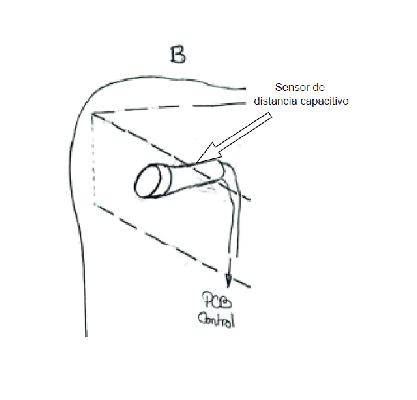
\includegraphics[width=.9\linewidth]{CHPTRS/CH03_DICON/Fig/CH03_FIG02_CoS/04d_CoSDibujosDeSeccion-B.pdf}
            \end{subfigure}
            \\
            % FILA-3 (captions superiores)
            \begin{subfigure}[t]{0.8\linewidth}
                \caption{Imagen del mecanismo general}
                \label{fig:imagen1}
            \end{subfigure}
            &
            \begin{subfigure}[t]{0.8\linewidth}
                \caption{Vista de sección}
                \label{fig:imagen2}
            \end{subfigure}
            \\
            % FILA-4 (captions inferiores)
            \begin{subfigure}[t]{0.8\linewidth}
                \caption{Detalle A del mecanismo}
                \label{fig:imagen3}
            \end{subfigure}
            &
            \begin{subfigure}[t]{0.8\linewidth}
                \caption{Detalle B del mecanismo}
                \label{fig:imagen4}
            \end{subfigure}
        \end{tabularx}
        \caption{Detalle de mecanismo de ajuste de motor \ac{DC}}
        \label{fig:detalle1}
    \end{figure}
    
    La desventaja de utilizar este mecanismo radica en que los motores \ac{DC} no deben sobreajustarse excesivamente, ya que esto puede ocasionar fallos mecánicos significativos. Un sobreajuste podría deformar la carcasa del motor, lo que a su vez podría desalinear componentes internos como el estator y el rotor. Esto generaría un aumento en la fricción durante el giro del eje, recordar que los componentes del motor son ensamblados de forma que se aproveche el campo magnético para generar el giro del rotor al paso de corriente (para visualizar las partes internas de un motor \ac{DC}, consultar la sec. \ref{sec:CH02_INTRODUCCION} del Anexo \ref{an:Anexo_C}). Este esfuerzo incrementado implica una mayor demanda de corriente, lo que reduce la eficiencia del sistema y puede llevar a un desgaste prematuro de los componentes internos.


\textbf{Solución 2: }   
    El sistema se alimentará de una fuente de $220\text{VAC }60\text{Hz}$ conectada al tomacorriente, e incluirá un botón de encendido y apagado en el chasis para activar los módulos internos. La disipación de calor se realizará mediante un ventilador. El estado de los diferentes módulos será visible a través de tres LEDs indicadores, de distintos colores, que representarán el estado de control, sensores y actuadores. Los estados para todos los dominios significará si está o no correctamente energizados los componentes electrónicos y cada dominio estará representado por un color.
    	
    Para la comunicación entre el \ac{HW} y la interfaz de usuario, se prescindirá de la comunicación serial directa, aunque podría habilitarse si fuera necesario. En su lugar, la transmisión de datos se realizará de forma remota mediante Wi-Fi, utilizando un \textit{broker} gratuito de mensajería bajo un estándar como \ac{MQTT}. Esto permitirá que el sistema se comunique con una aplicación web. Esta solución estará pensada para casos donde se requiera acceso y monitoreo remoto. Esta estructura elimina la dependencia de conexiones seriales físicas, aunque está sujeta a la disponibilidad de conexión a internet durante el proceso de estimación. La desventaja de usar la comunicación por \ac{MQTT} es que el \textit{broker}, que sirve como medio entre el \ac{HW} encargado del sensado y la interfaz, puede saturarse al tener que recibir y procesar información proveniente de tres sensores distintos, especialmente si los datos se envían con alta frecuencia o en grandes volúmenes. Esto podría ocasionar retrasos en la entrega de mensajes, pérdida de información o incluso un fallo total del sistema si el \textit{broker} no está correctamente configurado para manejar la carga.
    El bosquejo de esta solución se presenta a continuación en la Figura \ref{fig:sol2_fuera}
    \begin{figure}[H]
        \centering
        \begin{tabularx}{\linewidth}{>{\centering\arraybackslash}X}
            % Fila 1: imagen
            \begin{subfigure}[t]{1\linewidth}
                \centering
                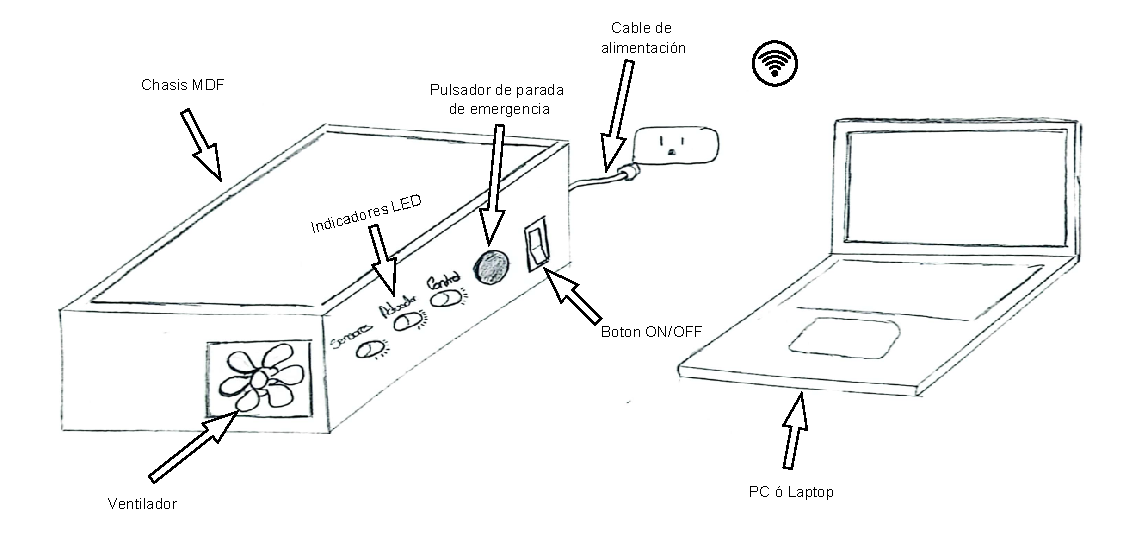
\includegraphics[width=\linewidth]{CHPTRS/CH03_DICON/Fig/CH03_FIG02_CoS/05_CoS_Solucion2porFuera.pdf}
            \end{subfigure}
        \end{tabularx}
        \caption{Concepto 2 - Vista desde afuera del \ac{HW} del sistema}
        \label{fig:sol2_fuera}
    \end{figure}
    
    
    En el diseño interno del \ac{HW}, se ha implementado un sistema de protección mediante una llave termomagnética en la entrada de potencia, asegurando la integridad de los componentes ante posibles sobrecargas. La alimentación de cada módulo se gestionará a través de un circuito rectificador y regulador diseñado específicamente para energizar cada sección del sistema. Se incluirán conectores y pistas de \ac{PCB} para distribuir eficientemente la alimentación, manteniendo un diseño compacto.
    En cuanto a la parte de lógica y control, se utilizará un microcontrolador con conectividad Wi-Fi. En caso de optar por un controlador sin dicha funcionalidad, se deberá acoplar un módulo Wi-Fi adicional para el envío de datos.     	
    \begin{figure}[H]
        \centering
        \begin{tabularx}{\linewidth}{>{\centering\arraybackslash}X}
            % Fila 1: imagen
            \begin{subfigure}[t]{\linewidth}
                \centering
                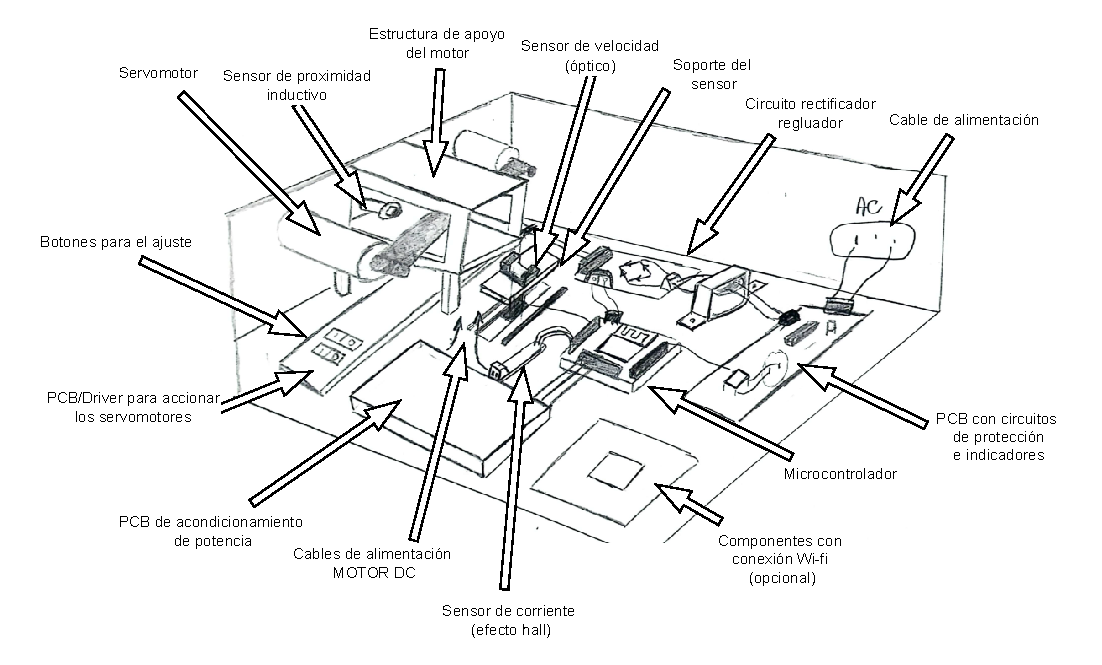
\includegraphics[width=\linewidth]{CHPTRS/CH03_DICON/Fig/CH03_FIG02_CoS/06_CoS_Solucion2porDentro.pdf}
            \end{subfigure}
        \end{tabularx}
        \caption{Concepto 2 - Vista desde adentro del \ac{HW} del sistema}
        \label{fig:sol2_dentro}
    \end{figure}
        
    El mecanismo de sujeción del motor para la estimación utilizará un sistema de correas y servomotores para asegurar la fijación necesaria. Este mecanismo será capaz de ajustar y sujetar el motor en su posición ideal de forma controlada.  El usuario será el encargado de ir ajustando o desajustando gradualmente las correas para asegurar al motor. Adicionalmente, se instalará un sensor de presencia inductivo que detectará la correcta colocación del motor antes de iniciar el proceso de estimación, garantizando una configuración segura y precisa.
    \begin{figure}[H]
        \centering
        \begin{tabularx}{\linewidth}{>{\centering\arraybackslash}X}
            % Fila 1: imagen
            \begin{subfigure}[t]{0.45\linewidth}
                \centering
                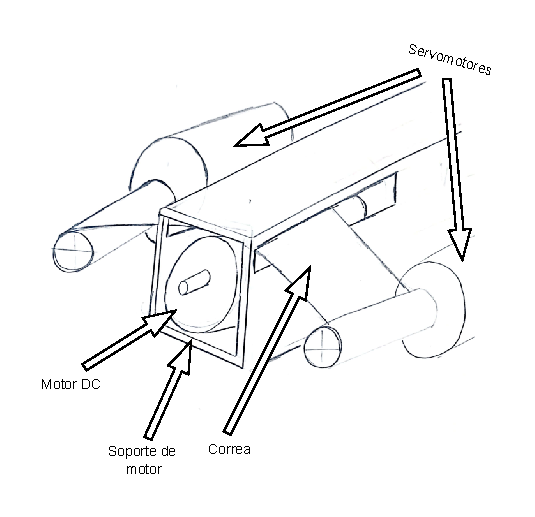
\includegraphics[width=\linewidth]{CHPTRS/CH03_DICON/Fig/CH03_FIG02_CoS/07_CoSAcopleDeCintas.pdf}
            \end{subfigure}
        \end{tabularx}
        \caption{Detalle de mecanismo de sujeción de motor \ac{DC} para la solución 2}
        \label{fig:CINTAS}
    \end{figure}
    
    Dado que la finalidad es analizar distintos tipos de motores dentro del rango de 12V, se busca estandarizar la medición de velocidad usando un disco ajustable que tenga ranuras para el sensado usando un sensor infrarrojo. El diseño de este consta de utilizar 3 tornillos de sujeción, esto inspirados en las sujeciones presentes en maquinas de manufactura como los tornos o fresadoras.  
    \begin{figure}[H]
        \centering
        \begin{tabularx}{\linewidth}{>{\centering\arraybackslash}X}
            % Fila 1: imagen
            \begin{subfigure}[t]{0.7\linewidth}
                \centering
                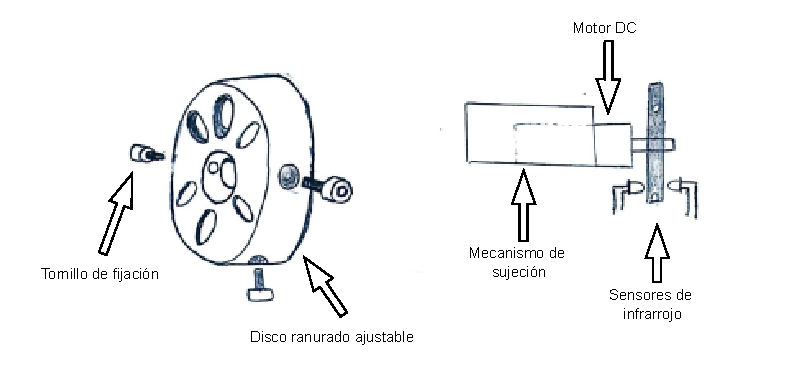
\includegraphics[width=\linewidth]{CHPTRS/CH03_DICON/Fig/CH03_FIG02_CoS/08_CoSAcopleOptico2.pdf}
            \end{subfigure}
        \end{tabularx}
        \caption{Acople de \textit{encoder} óptico ajustable a distintos diámetros de motor}
        \label{fig:acople_op_2}
    \end{figure}


\textbf{Solución 3:}
    Para esta solución, el sistema se alimentará directamente desde un tomacorriente de $220 \text{VAC}$ y $60 \text{Hz}$. La comunicación entre el \ac{HW} y el \ac{SW} se llevará a cabo mediante un enlace serial a través de Ethernet, el cual ofrece alta resistencia al ruido y asegura una transferencia de datos de calidad. Su velocidad y fiabilidad garantizan un rendimiento óptimo, y el acceso a esta comunicación estará disponible en el chasis del dispositivo. A diferencia de la solución anterior, no se requerirá comunicación remota. En esencia, el funcionamiento de esta propuesta es similar al primer concepto de solución, con ligeras modificaciones, destacando la inclusión de un módulo para habilitar la comunicación Ethernet.
    
    El chasis y las piezas de apoyo serán construidos mediante impresión 3D, para  incluir de manera sencilla  ranuras o estructuras específicas que acomoden los diferentes módulos y componentes que conformarán la solución, en especial los componentes internos del sistema. Para disipar el calor generado en los puntos de alta potencia, tales como la fuente reguladora de \ac{AC}/\ac{DC} o los \textit{drivers} de motor, se integrarán disipadores de calor en las áreas correspondientes del chasis. Esto ayudará a mantener una temperatura óptima en el interior del sistema y evitará el sobrecalentamiento de los circuitos sin recurrir al uso de un ventilador que significará un gasto constante de energía por parte del sistema. 
    
    Al igual que las soluciones anteriores, se incluirán indicadores LED que mostrarán el estado de funcionamiento de los tres módulos del \ac{HW} y contará con  los botones necesarios para la operación y seguridad, incluyendo un botón de encendido y apagado y un botón de parada de emergencia, el cual permitirá al usuario desactivar el sistema de forma inmediata en caso de cualquier problema.
        
    \begin{figure}[H]
    \centering
    \begin{tabularx}{\linewidth}{>{\centering\arraybackslash}X}
        % Fila 1: imagen
        \begin{subfigure}[t]{1\linewidth}
            \centering
            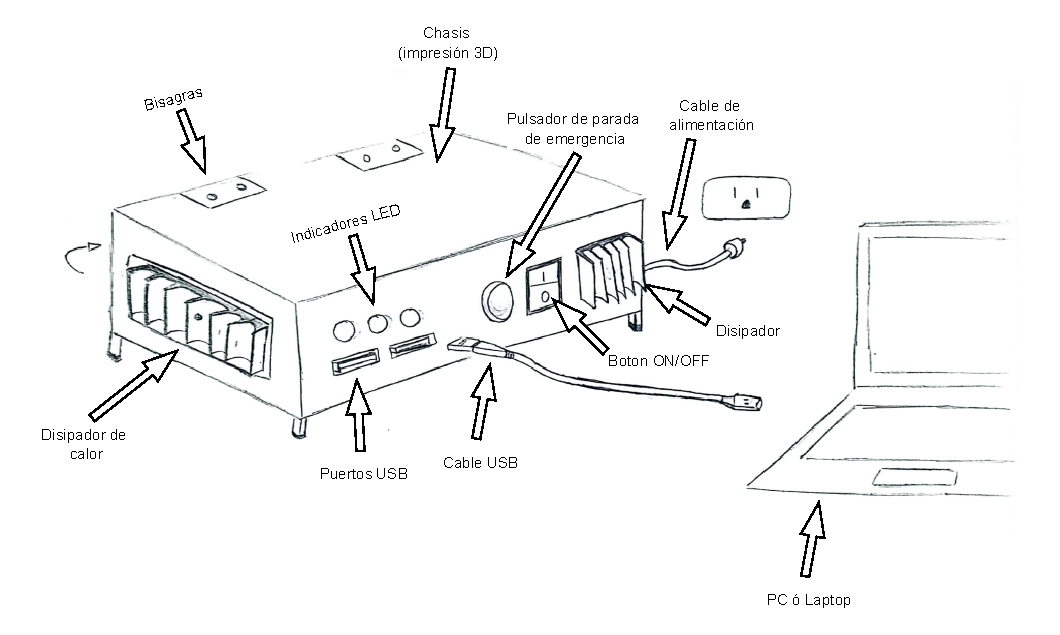
\includegraphics[width=\linewidth]{CHPTRS/CH03_DICON/Fig/CH03_FIG02_CoS/09_CoS_Solucion3porFuera.pdf}
        \end{subfigure}
    \end{tabularx}
    \caption{Concepto 3 - Vista desde afuera del \ac{HW} del sistema}
    \label{fig:sol3_fuera}
    \end{figure}
    
    En cuanto al diseño de los circuitos internos, se ha previsto un sistema de protección adicional mediante relés electromagnéticos, los cuales protegerán el sistema contra posibles sobrecargas eléctricas.
    Se propone diseñar soportes específicos para cada uno de los motores a utilizar, tomando como referencia los dibujos técnicos contenidos en sus respectivas fichas técnicas. Dichos dibujos siguen normas estandarizadas de montaje, por lo que, si bien no se busca desarrollar un acople universal, los diseños respetarán los estándares propios de cada motor. Sin embargo, la medida que sí se puede estandarizar son la distancia entre agujeros de sujeción con la mesa de pruebas, la cual contará con ranuras fijas para el ajuste de los motores dependiendo de qué tan extensos sean los motores a evaluar. En la Figura \ref{fig:soporte_motor} se muestra un boceto preliminar del diseño del soporte propuesto para los motores motores y en la Figura \ref{fig:base} se muestra la base donde se fijará el motor.
    \begin{figure}[!ht]
    \begin{tabularx}{\linewidth}{*{2}{>{\centering\arraybackslash}X}}
        % FILA-1 (imágenes)
        \begin{subfigure}[t]{0.35\textwidth}
            \centering
            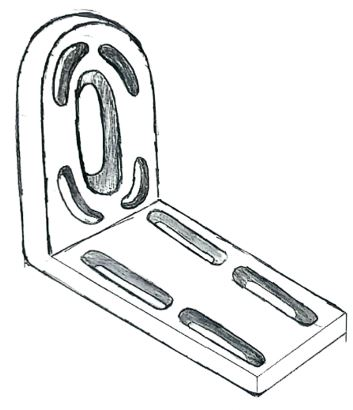
\includegraphics[width=.7\linewidth]{CHPTRS/CH03_DICON/Fig/CH03_FIG02_CoS/10a_CoS_SoporteDeMotor.JPG}
        \end{subfigure}
        &
        \begin{subfigure}[t]{0.35\textwidth}
            \centering
            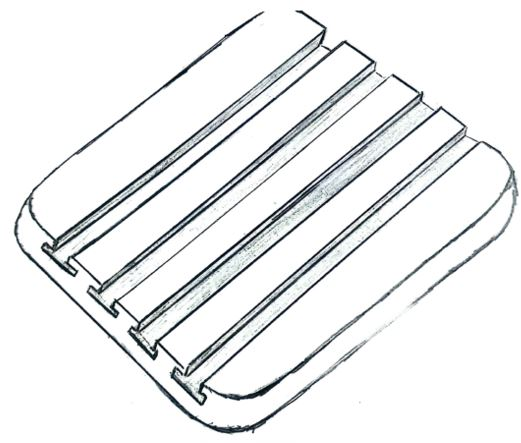
\includegraphics[width=.7\linewidth]{CHPTRS/CH03_DICON/Fig/CH03_FIG02_CoS/10b_CoS_BancoDeEnsayo.JPG}
        \end{subfigure}
        \\
        % FILA-2 (captions)
        \begin{subfigure}[t]{0.8\linewidth}
            \caption{Soporte para motores \ac{DC}}
            \label{fig:soporte_motor}
        \end{subfigure}
        &
        \begin{subfigure}[t]{0.8\linewidth}
            \caption{Mesa ranurada donde se fijará el motor}
            \label{fig:base}
        \end{subfigure}
    \end{tabularx}
    \caption{Piezas para la fijación del motor}
    \label{fig:sistema_acople_motor_sol3}
    \end{figure}
    
    Otro de los cambios más importante en esta solución, respecto a las demás, es el tipo de sensor de velocidad empleado. En lugar de un \textit{encoder} óptico, se ha optado por un \textit{encoder} basado en efecto Hall, que detectará la rotación de un disco acoplado al eje de salida del motor. Este disco estará equipado con imanes que permitirán al \textit{encoder} enviar la información al controlador del paso de estos imanes y por ende la medición de velocidad del motor. 
    A continuación se presenta el bosquejo de una vista interior del \ac{HW} del sistema. La disposición y montaje del sensor de velocidad, con el \textit{encoder} y el disco magnético, se presenta con un ejemplo en la Figura \ref{fig:IMAGENES_XTRAS}, donde se utiliza sensores de efecto Hall para el sensado de velocidad de un motor.
    \begin{figure}[H]
    \centering
    \begin{tabularx}{\linewidth}{>{\centering\arraybackslash}X}
        % Fila 1: imagen
        \begin{subfigure}[t]{1\linewidth}
            \centering
            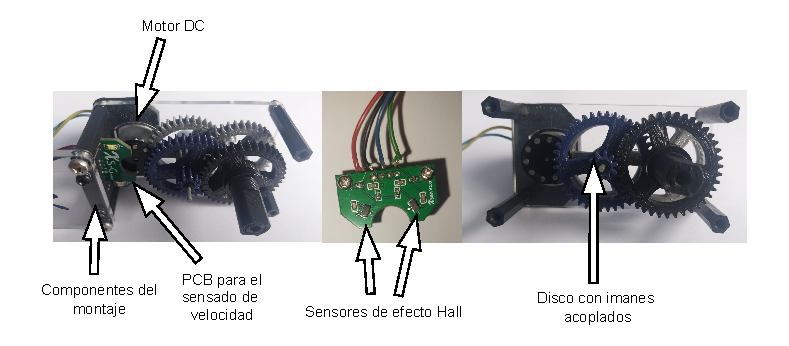
\includegraphics[width=\linewidth]{CHPTRS/CH03_DICON/Fig/CH03_FIG02_CoS/11_CoS_ImagenesExtraSolucion3.pdf}
        \end{subfigure}
        \\[2mm]
        % Fila 2: nota
        \begin{subfigure}[t]{\linewidth}
            \caption*{\textit{Imágenes tomadas de un módulo educativo, cortesía del ingeniero Celso de la Cruz}}
        \end{subfigure}
    \end{tabularx}
    \caption{Montaje de un \textit{encoder} magnético en el eje del motor.}
    \label{fig:IMAGENES_XTRAS}
    \end{figure}
    
    Utilizando el ejemplo mostrado, se puede diseñar un disco con imanes acoplados que se ajuste a un amplio rango de diámetros de eje de motor, similar a lo presentado en el segundo concepto. En la Figura \ref{fig:acople_magn} se muestra una comparación entre las 2 ideas de solución para medir la velocidad del motor. En la segunda se ha dibujado el disco ajustable a diferentes diámetros similar a la solución anterior.
    \begin{figure}[H]
    \centering
    \begin{tabularx}{\linewidth}{>{\centering\arraybackslash}X}
    % Fila 1: imagen
    \begin{subfigure}[t]{0.6\linewidth}
        \centering
        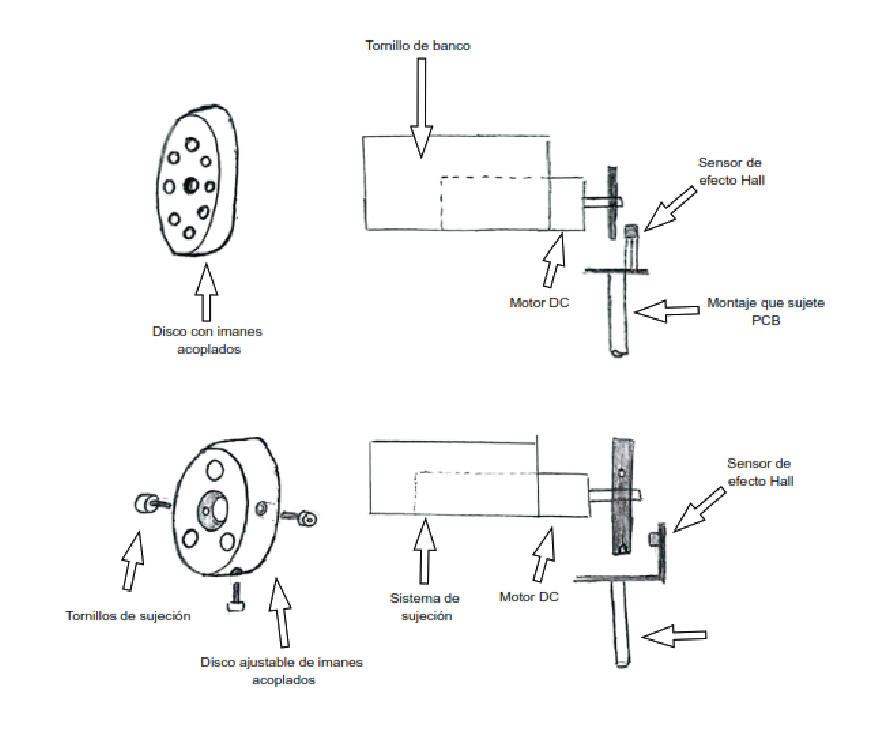
\includegraphics[width=\linewidth]{CHPTRS/CH03_DICON/Fig/CH03_FIG02_CoS/12_CoS_AcopleMagnetico.pdf}
    \end{subfigure}
    \end{tabularx}
    \caption{Acople de \textit{encoder} magnético ajustable a distintos diámetros de motor}
    \label{fig:acople_magn}
    \end{figure}
    
    Finalmente, se muestra el interior del concepto de solución 3 en la Figura \ref{fig:sol3_dentro}.
    \begin{figure}[H]
    \centering
    \begin{tabularx}{\linewidth}{>{\centering\arraybackslash}X}
    % Fila 1: imagen
    \begin{subfigure}[t]{0.8\linewidth}
        \centering
        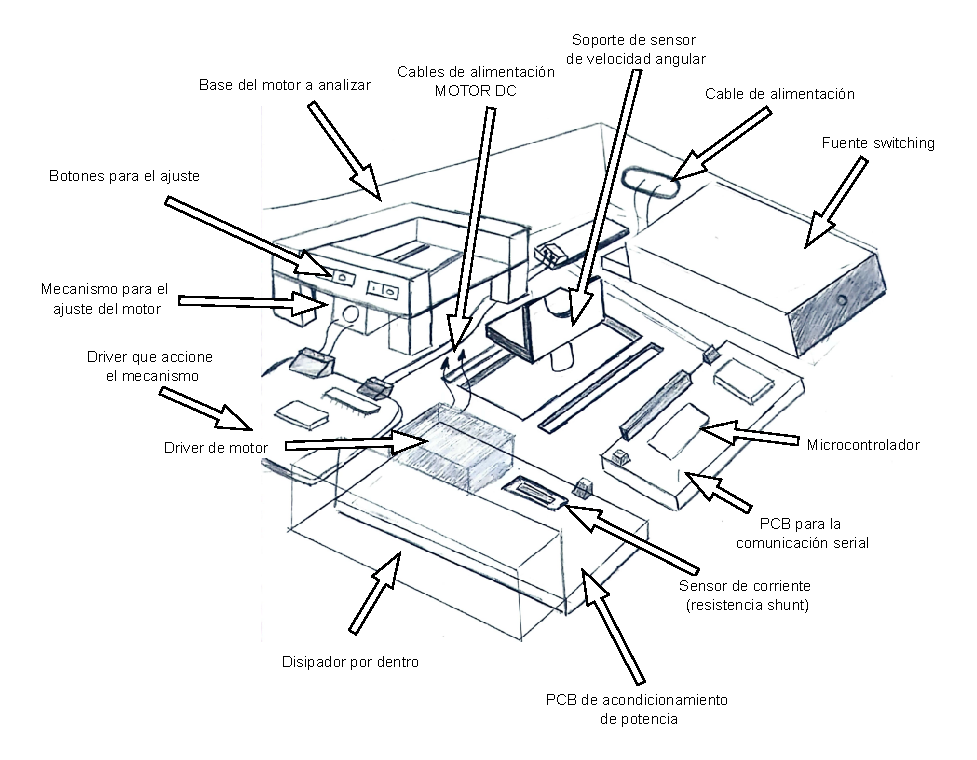
\includegraphics[width=\linewidth]{CHPTRS/CH03_DICON/Fig/CH03_FIG02_CoS/13_CoS_Solucion3porDentro.pdf}
    \end{subfigure}
    \end{tabularx}
    \caption{Concepto 3 - Vista desde adentro del \ac{HW} del sistema}
    \label{fig:sol3_dentro}
    \end{figure}

